\startchapter{Mixture of Molecules} \label{ch:5}
\section{Description}

In Chapter \ref{ch:4}, test cases indicate that for one type of molecule at interfaces, even combining all the three spectral information, the constructed LP model cannot return the target composition in most cases. The existing spectral information is not adequate to obtain the target composition of one type of molecule at interfaces. Multiple return compositions can build the spectra that are almost exactly the same as the target ones. These compositions are returned by the LP models that use different amounts of spectral information. This indicates that even extracting data information from three spectroscopy techniques, it is still not sufficient to obtain the target composition for one type of molecule at interfaces. Besides one type of molecule at interfaces, we are also interested in the case where different molecules at interfaces. For a mixture of different molecules at interfaces, we want to figure out whether our LP model can help to obtain the target composition. If the LP model success in obtaining the target composition with certain spectral information, we want to know which spectral information. Moreover, we want to know the efficiency of the spectral information in obtaining the target composition. \\

\section{Test Cases}
\subsection{Test Cases Considering Each Amino Acid Candidates from $0^{\circ}$ to $80^{\circ}$ on $\theta$ in the Mixture}
To achieve the study of the orientation distribution of various molecules at interfaces, further test cases are constructed. These test cases have the following common settings. \\

First, there are six different amino-acids in the mixture: methionine, leucine, isoleucine(ile), alanine, threonine and valine. For each amino acid, only $\theta$ difference is considered, the other two Euler angles are integrated. Each amino acid molecule has 9 candidates in the mixture, they have $\theta$ of the following values: $0^{\circ}$,  $10^{\circ}$, $20^{\circ}$, $30^{\circ}$, $40^{\circ}$, $50^{\circ}$, $60^{\circ}$, $70^{\circ}$ and $80^{\circ}$. Because when $\theta$ equals $90^{\circ}$, the SFG spectra is a straight line. The corresponding candidate is excluded from all the test cases. As a result, there are 54 candidates in the mixture. \\

Second, the target composition need to be generated. The operation includes two steps: randomly pick one candidate from each amino acid's 9 candidates, then randomly generate a percentage for the selected candidate. The target composition is made of six randomly selected candidates with assigned percentage coming from the amino acids. The rest $48$ candidates have $0$ percentage in the target composition. Namely, six selected candidate makes 100\% component of the mixture. \\

Third, the IR, Raman and SFG spectra need to be generated for all the $54$ candidates and the target. \\

Table \ref{tab:5.1} displays a set of test cases, each test case contains different spectral information. In Case 1, candidates $x$- and $z$-polarized IR spectra are obtained. The target's IR spectra are generated by the dot product of the target composition and all the candidates' spectral data. Then the corresponding LP model is conducted using Equation \ref{eq:3.4}. Therefore, we claim that the LP model in Case 1 only contains IR information.\\

\begin{table}
\begin{center}
{\def\arraystretch{1.5}
\begin{tabular}{| l | p{3in} | }
\hline
Test Case Index & Spectral Information \\
\hline
Case 1 & $x$ and $z$ polarized IR spectra\\
\hline
Case 2 & $xx$, $xy$, $xz$ and $zz$ polarized Raman spectra \\
\hline
Case 3 & $xxz$, $xzx$ and $zzz$ polarized SFG spectra \\
\hline
Case 4 & $x$ and $z$ polarized IR spectra \newline $xx$, $xy$, $xz$ and $zz$ polarized Raman spectra \\
\hline
Case 5 & $x$ and $z$ polarized IR spectra \newline $xxz$, $xzx$ and $zzz$ polarized SFG spectra \\
\hline
Case 6 & $xx$, $xy$, $xz$ and $zz$ polarized Raman spectra \newline $xxz$, $xzx$ and $zzz$ polarized SFG spectra \\
\hline
Case 7 & $x$ and $z$ polarized IR spectra \newline
 $xx$, $xy$, $xz$ and $zz$ polarized Raman spectra \newline 
 $xx$, $xzx$ and $zzz$ polarized SFG spectra \\
\hline
\end{tabular} 
}
\end{center}
\caption{Detailed test cases set setting for the mixture of amino acids} 
\label{tab:5.1} 
\end{table}	

Similarly, Case 2 contains only Raman spectral information of the following four polarizations: $xx$, $xy$, $xz$ and $zz$. Case 3 contains only SFG spectral information of $yyz$, $yzy$ and $zzz$ three polarizations. \\

Starting from Case 4, spectral information of different spectroscopy techniques are combined. In Case 4, IR spectral information is combined with Raman. In Case 5, IR spectral information is combined with SFG. In Case 6, Raman and SFG spectral information are incorporated. At the end, in Case 7, all three spectral information are put together: IR, Raman and SFG. \\

Finally, this test case set is run 100 times in order to see which case in the set returns the target composition with the highest accuracy. This accuracy is measured by the time of each case returns the target composition. The scoring mechanism to measure whether a return composition matches to the target one is described in the next section. \\

\subsection{Scoring method}

At the first glance, the sum of residuals between the spectra composed by the return composition and the target one can be used to measure the accuracy of the return composition. However, in most test cases conducted earlier, the spectra generated by the return composition are almost identical to the ones created by the target composition. The sum of residuals between these spectra is negligible, which makes it appropriate to use as a scoring criteria. \\

Another way to measure the accuracy of the return composition, is to compare it directly with the target one. Calculating the sum of the residuals between a target composition and a return one directly can be a fast approach to evaluate the accuracy of each case. The shortage of this approach is that it cannot be used to measure in realistic test cases where the target composition is unknown. However, in the current test cases, this approach can be a way to evaluate the return composition for all the test cases where the target compositions are known in advance. \\

The return composition of each test case in the set is obtained for each run. Each return composition is compared with the target one to calculate the sum of the residuals. If the sum is smaller than a certain threshold, which is $10^{-7}$, then the return composition is considered to be the same as the target one. \\

\begin{figure}[!ht]
\centering
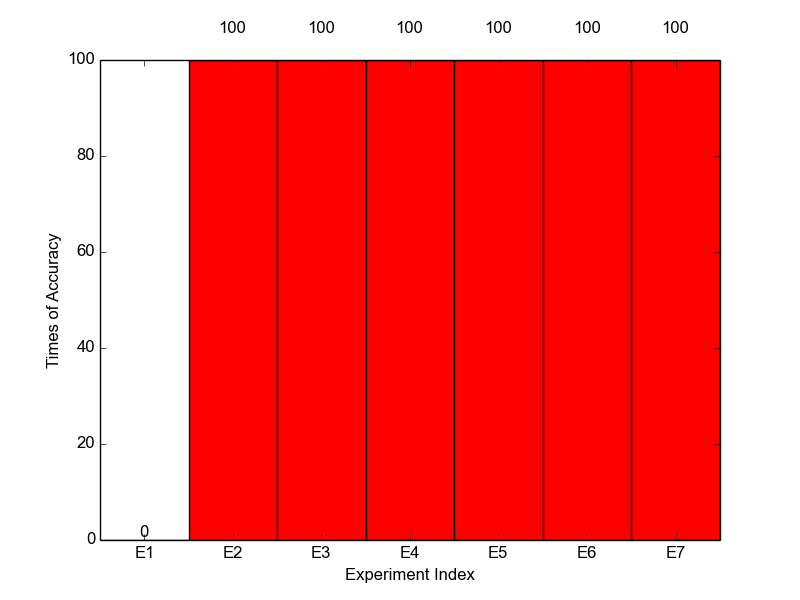
\includegraphics[scale=0.7]{Figures/accuracy_pecent_result8_mixture.png}
\caption{Accuracy analysis for test cases considering a mixture of amino acids with candidates from $0^{\circ}$ to $80^{\circ}$ on $\theta$ for each amino acid. Accuracy indicates how many times each test case in the set return a composition matches the target one.}  \label{fig:5.1}
\end{figure}

The test case set is run 100 times based on the scoring method, the result is shown in 
Figure \ref{fig:5.1}. Case 2, 3, 4, 5, 6 and 7, all return the target composition in the 100 runs. This result indicates that Raman or SFG alone is sufficient to obtain the target composition. For a mixture of amino acids with candidates from $0^{\circ}$ to $80^{\circ}$ on $\theta$ for each amino acid. Any test cases that contain Raman and SFG result in the same accuracy. \\

The only exception is Case 1. The accuracy is fairly low, which indicates that IR spectra do not contain sufficient information in order to obtain the target composition. \\

To take a further insight into the return composition of Case 1, the test case set is re-run 100 times, only the return composition of Case 1 is analyzed and focused. In each run, IR $x$- and $z$-polarized spectra are plotted both by the returned composition and the target one. The result is that these spectra conducted by the two different compositions are very close to each other in each run. Randomly take one run as an example, Figure \ref{fig:5.2} displays the plotted spectra, and they are almost identical to each other. The residual is very small for the data points where these two spectra are not overlapped. This indicates that the optimum composition returned by the LP model conducted with only IR spectral information has achieved its best in obtaining a composition that best fit the target spectra. 

(TODO: rewrite or remove this paragraph) Comparatively, SFG has three unique polarizations, and Raman has four unique polarizations. From each projection's spectrum, we evenly select 200 data points. This means that one more projection will bring in 200 more constraints or 400 more (when we take the absolute sign off) constraints to the LP model. This would make a huge difference in the LP model, in term of further refining the candidate selection in target composition. However, it is still too early for us to say that Raman has more orientation information because it has four unique polarizations. Because for Raman's any polarization, the spectrum of candidate with $\theta$ equals to one degree is identical to the one of candidate with this $\theta$ degree's complementary. For example, the Raman spectra for candidate with $\theta$ of $10^{\circ}$, is the same as candidate with $\theta$ of $170^{\circ}$. And for IR, it is the same case. Only SFG tells the differences between these two degrees, as the spectra for candidate with $\theta$ of one degree is symmetric to its complementary along wavenumber as shown in Figure \ref{fig:5.8}. \\

\begin{figure}[!ht] 
\centering
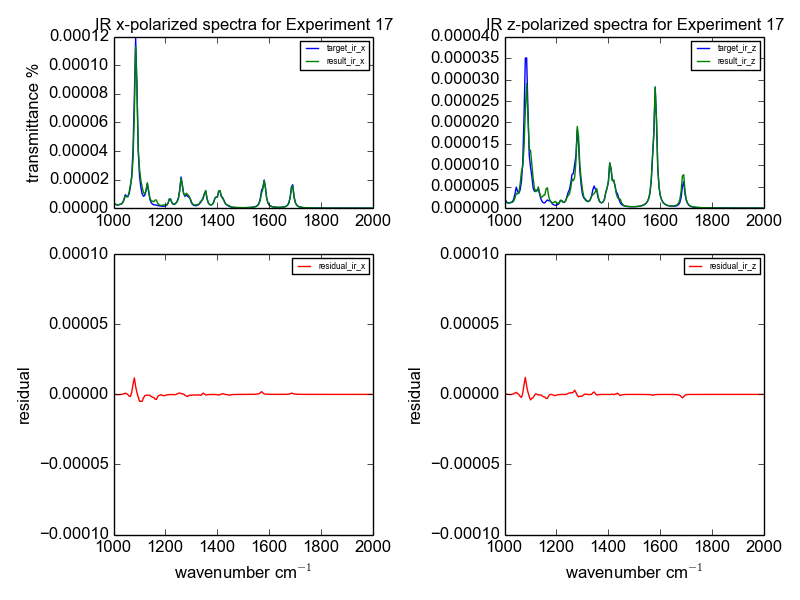
\includegraphics[scale=0.7]{Figures/chapter5_result_target_residual_plotting__ir_result8_run1.png}
\caption{IR spectra plotted by the result composition and the target composition of one ramdon run when considering each amino acid candidates from $0^{\circ}$ to $80^{\circ}$ on $\theta$ in the Mixture.} \label{fig:5.2}
\end{figure}

\subsection{Test Cases Considering Each Amino Acid Candidates from $0^{\circ}$ to $180^{\circ}$ on $\theta$ in the Mixture}
To further study the capacity of the LP models built for the mixture of molecules,the candidate pool is expanded from $0^{\circ}$ to $180^{\circ}$ in terms of the $\theta$ value. Therefore, each amino acid has $18$ candidates. In total, there are $108$ candidates in the mixture. The same set of test cases in Table \ref{tab:5.1} is used. The only difference is instead of randomly select one candidate from $9$ candidates, it is selected from $9$. All $108$ candidates' IR, Raman and SFG spectra need to be generated. Figure \ref{fig:5.3} illustrates the results obtained in $100$ runs. The accuracy in Case 1 is still low. This is not surprising as the complexity of the candidates has increased. Moreover, IR spectra for candidate with $\theta$ of one degree is identical to the one with $\theta$ of this degree's complementary, as shown in Figure \ref{fig:A.1}. This also increases the difficulty for the LP model using IR spectral information to return the target composition. \\

\begin{figure}[!ht]
\centering
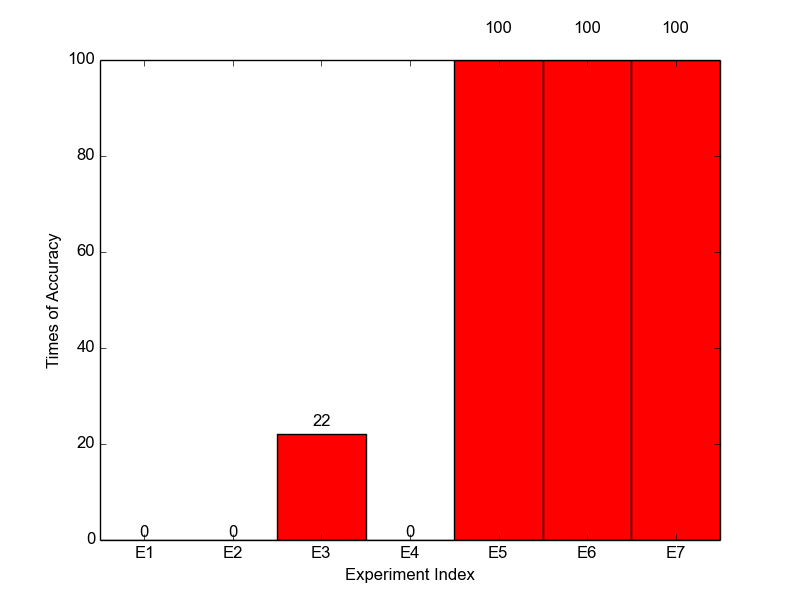
\includegraphics[scale=0.7]{Figures/accuracy_pecent_result10_mixture.png}
\caption{Accuracy analysis for test cases considering a mixture of amino acids with candidates from $0^{\circ}$ to $180^{\circ}$ on $\theta$ for each amino acid. Accuracy indicates how many times each test case in the set return a composition matches the target one.} \label{fig:5.3}
\end{figure}

However, it should be noticed that the accuracy for Case 2 has dramatically dropped. This can be caused by the Raman spectra for one candidate with a $\theta$ is identical to the one of this $\theta$ value's complementary as displayed in Figure \ref{fig:A.2}. \\

In Figure \ref{fig:5.3}, the accuracy for Case 3 is no longer high neither. After increasing the number of amino acid candidates from $9$ to $18$, the complexity of the corresponding LP model has increased. Although the added candidates' SFG spectra are symmetric along wavenumber which may greatly increase the uniqueness of the candidates as shown in Figure \ref{fig:A.3}. The SFG spectral information is still insufficient to obtain the target composition. \\

The good result starts to emerge when using the combinations of IR and SFG or Raman and SFG. Figure \ref{fig:5.3} shows that Case 5, 6, and 7 all have 100\% accuracies. This phenomenon can be explained as follow: SFG helps to distinguish a candidate from its complementary on $\theta$ value. The extra spectral information coming from IR or Raman helps to further refine the LP model, which can then converge the return composition to the target one. \\

Although the accuracy in Case 2 is low. There is still some noticable result in the return composition: for each amino acid, the percentage assigned is correct; however, the candidate presented may be always be correct. It is either the correct one, or the correct one's complementary. Randomly select one test case run as an example, Figure \ref{fig:5.4} displays the target composition. Figure \ref{fig:5.5} displays the return composition of Case 2 in the run. Figure \ref{fig:5.6} is the return composition of Case 6. Figure \ref{fig:5.4} and \ref{fig:5.6} are identical, which means the return composition of Case 6 is the same as the target one. The values in Figure \ref{fig:5.5} are the same as Figure \ref{fig:5.4}. However, the position of each value is not the same in two the figures. For example, the percentage value $0.299586$ of methionine is for $\theta = 120^{\circ}$ in Figure \ref{fig:5.4}, but is for $theta = 60^{\circ}$ in Figure \ref{fig:5.5}. These two angles are complementary. This observation is the same for isoleucine, alanine, threonine, and valine in the figure. This observation is a general case across all the runs of the test case set. The return composition of Case 6 matches the target one. However, the return composition of Case 2 fails to pick each amino acid's correct candidate from this candidate's complementary. This can be explained as the Raman spectra for one $\theta$ are the same as its complementary. \\

\begin{figure}[!ht] 
\centering
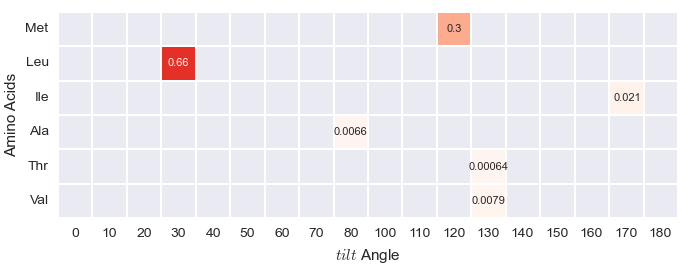
\includegraphics[scale=0.9]{Figures/mixture_target_composition_for_one_run_theta_0_180.png}
\caption{Target composition of one random run of six mixed amino acids with candidates expanded from $0^{\circ}$ to $180^{\circ}$ on $\theta$ for each amino acid. More detailed data of this target composition can be found in Appendix \ref{eqn:A.1}. } 
\label{fig:5.4}
\end{figure}

\begin{figure}[!ht] 
\centering
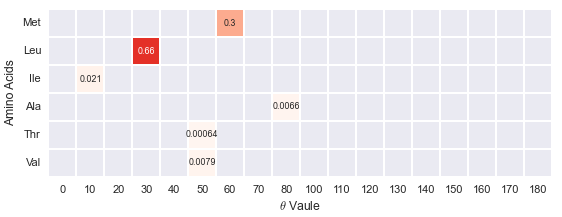
\includegraphics[scale=0.9]{Figures/mixture_return_composition_of_E1_for_one_run_theta_0_180.png}
\caption{Return composition of Case 2 for one random run of six mixed amino acids with candidates expanded from $0^{\circ}$ to $180^{\circ}$ on $\theta$. More detailed data of this return composition can be found in Appendix \ref{eqn:A.2}.} 
\label{fig:5.5}
\end{figure}

\begin{figure}[!ht] 
\centering
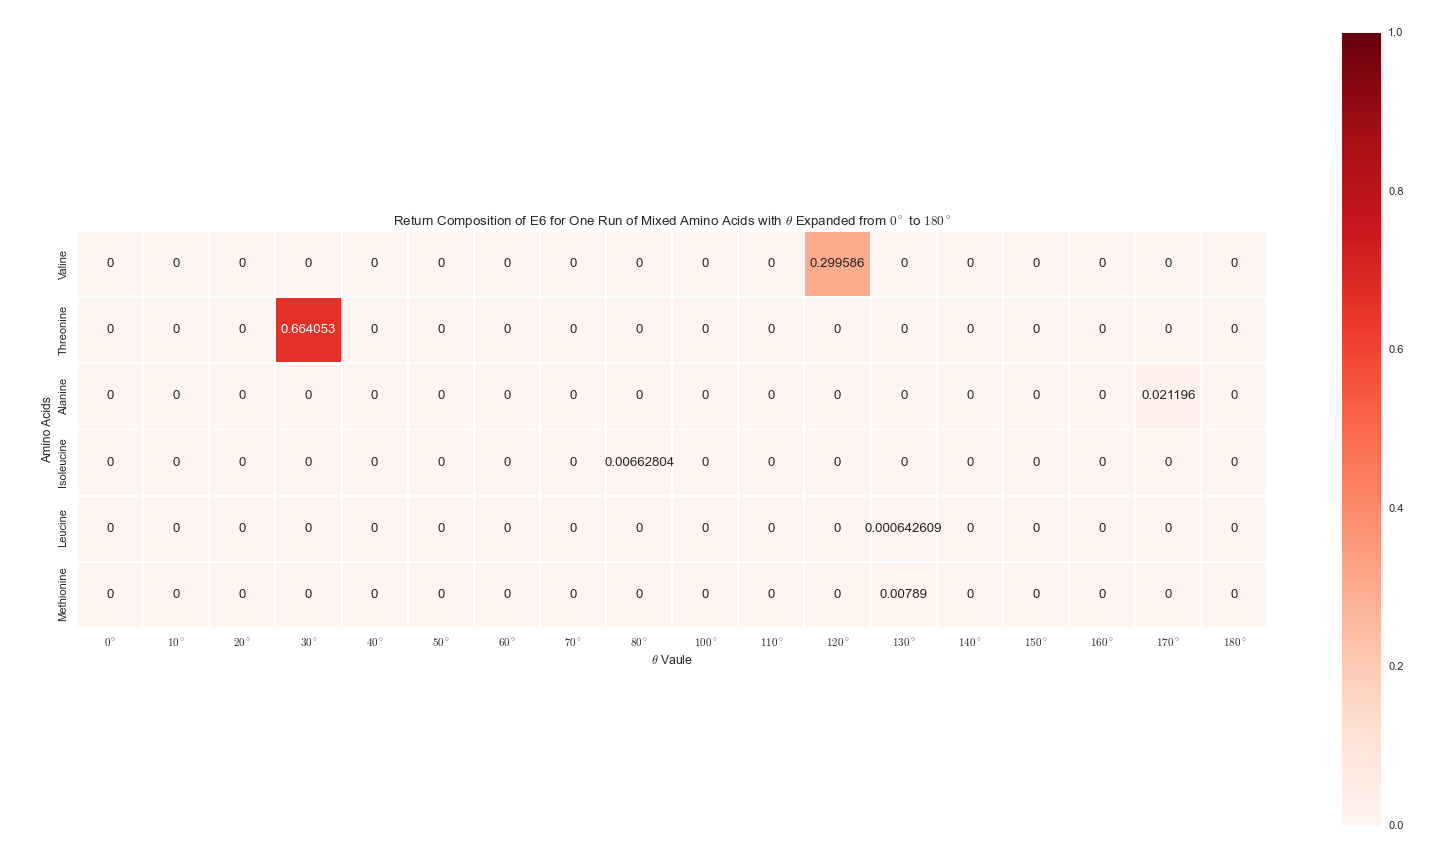
\includegraphics[scale=0.9]{Figures/mixture_return_composition_of_E6_for_one_run_theta_0_180.png}
\caption{Return composition of Case 6 for one random run of six mixed amino acids with candidates expanded from $0^{\circ}$ to $180^{\circ}$ on $\theta$. More detailed data of this return composition can be found in Appendix \ref{eqn:A.3}.} 
\label{fig:5.6}
\end{figure}

The return composition of Case 4 is the same as the one of Case 2, which means combining IR spectra information with Raman is not sufficient for this test cases setting. This is because the IR spectra for one $\theta$ degree are also the same as its complementary. Spectral information from SFG is needed in order to study the cases that having $\theta$ expanded from $0^{\circ}$ to $180^{\circ}$. \\


\section{Conclusion}
Raman and SFG spectral information alone is sufficient to obtain the target composition, when considering a mixture of amino acids with candidates expanded from $0^{\circ}$ to $80^{\circ}$ on $\theta$ for each amino acid. \\

When the candidates are expanded from $0^{\circ}$ to $180^{\circ}$ on $\theta$, SFG spectral information needs to combine with IR or Raman in order to obtain the target composition. \\
